\documentclass{article}

\usepackage{amsmath}
\usepackage{graphicx}

% if you need to pass options to natbib, use, e.g.:
% \PassOptionsToPackage{numbers, compress}{natbib}
% before loading nips_2016
%
% to avoid loading the natbib package, add option nonatbib:
% \usepackage[nonatbib]{nips_2016}

\PassOptionsToPackage{numbers,sort&compress}{natbib}
\usepackage[final]{nips_2016} % produce camera-ready copy
\usepackage[utf8]{inputenc} % allow utf-8 input
\usepackage[T1]{fontenc}    % use 8-bit T1 fonts
\usepackage{hyperref}       % hyperlinks
\usepackage{url}            % simple URL typesetting
\usepackage{booktabs}       % professional-quality tables
\usepackage{amsfonts}       % blackboard math symbols
\usepackage{nicefrac}       % compact symbols for 1/2, etc.
\usepackage{microtype}      % microtypography
\usepackage{float}

\title{Species Distribution Modelling using Presence-Only Data}


% The \author macro works with any number of authors. There are two
% commands used to separate the names and addresses of multiple
% authors: \And and \AND.
%
% Using \And between authors leaves it to LaTeX to determine where to
% break the lines. Using \AND forces a line break at that point. So,
% if LaTeX puts 3 of 4 authors names on the first line, and the last
% on the second line, try using \AND instead of \And before the third
% author name.

\author{
  s2274544\\
  %% examples of more authors
  \And
  s2222962\\
 \And
  s2145762\\
  \And
  s2859612 
}

\begin{document}

\maketitle

\begin{abstract}\vspace{-0.4em}
In this report, we used citizen science data to train a range of Species Distribution Models, and assess the effect of both the classification algorithm and the method used to generate pseudo-absence data on model
performance. %The best performing models utilise ensembles of decision trees, and we obtain statistically significant improvements in test performance when we use bias-informed pseudo-absence generation. 
%The most effective model obtained was a Random Forest model trained using one-vs-rest pseudo-absences, which achieved a median test AUC-ROC score of 0.949 across the 40 species tested.
All models performed better when trained using one-vs-rest pseudo-absence data instead of uniformly generated pseudo-absences. The most effective model was a Random Forest, which achieved a mean test AUC-ROC of 0.932 across the 40 species tested.
\end{abstract}

\section{Introduction}\vspace{-0.5em}
This study investigates modelling species distributions using presence-only data collected from citizen scientists (members of the public who collect scientific data). Species Distribution Models (SDMs) are designed to predict whether a species is present at a given location based on particular environmental characteristics. Our study constructs and evaluates SDMs trained on environmental features at the locations of given observations, examining how different models perform under various pseudo-absence generation strategies \cite{SDM_tutorial}.

The study of the distribution of organisms is of high importance within the field of ecology. For example, predicting the presence of particular species can allow us to identify sites that may be suitable for species reintroductions. A stronger understanding of species distributions will allow us to more accurately identify risks to endangered species, potentially aiding us in preventing future extinctions. An especially important application is predicting distribution change in species in response to changes in climate or land use. If we can quickly and accurately quantify how such anthropogenic changes impact an ecosystem, we will have stronger evidence for which scientific, political, or economic actions might need to be taken to prevent harm to critical ecosystems \cite{presence_absence_value}.

We attempt to address two main challenges in this report, both  arising from the citizen science nature of this dataset. The first and more fundamental challenge is the lack of absence observations, which makes the construction of a classifier less natural. We are able to draw from the significant literature on presence-only SDMs to address this \cite{Elith_2006} \cite{Elith_2022}. We also attempt to address the geographic bias of our observation data by proposing an alternative absence generation method.

Both the existing and proposed methods for handling absence data will be tested, alongside a brief analysis of different model types. Ultimately, this study aims to build on existing SDM methods while handling the challenges presented by presence-only citizen science data.

\section{Data Preparation}\vspace{-0.3em}

\subsection{Species Data}\vspace{-0.3em}
% I think we need to mention where the test data is/where it is from here 

All species-specific data was collected from two datasets, one of which was used for training and the other for testing. The training data, sourced via online social network iNaturalist \cite{inat}, includes geographical coordinates in which different species have been observed. All of this data is collected via citizen scientists. This data contains four key attributes; the latitude and longitude in which the observation was recorded, along with the species name and identification number. This dataset contains 272,037 observations globally across 500 different species. The country containing the highest number of observations is the United States, with 85,376 total records and 112 unique species. Given the high observation count and availability of externally sourced data for this region, we focus our study solely on species observed within the continental US. Another important aspect of our data is that the counts of species are not equal, with the minimum number of observations of a particular species being 50 and the maximum 2000. 

On the other hand, the test data, sourced via the International Union for Conservation of Nature and Natural Resources \cite{iucn}, includes a grid-like set of locations for all species from the training data. Instead of containing presence or absence labels, this dataset specifies, for each species, the indices of locations where it is known to be present. All other locations are then treated as absences. This is a key difference from the training set, which only includes presence data. Attributes in the test dataset, like the training set, include latitude, longitude, species name and identification number. Within the United States, the testing set contains 124,710 records across 138 species. \vspace{-0.6em}

\subsection{Introduction to External Data}\vspace{-0.6em}
In addition to the given species observation data, environmental features were obtained to form SDMs. These features were sourced from NCEI \cite{ncei2020}, SimpleMaps \cite{simplemaps2020}, the USDA \cite{usda2022} and the NACIS \cite{nacis2020}. Information on these features are provided in Appendix \ref{app:environmental features}. 

Species coordinates were used to find the distance to the nearest coastline, and to extract the proportion of farmland in the surrounding area (the given county) of where the observation was recorded, both of which were used as features. The remaining environmental features; temperature, precipitation, soil moisture, windspeed and NDVI, were joined to each observation by selecting the nearest (geographically) available feature measurement. This method ensures there are no records missing from our data. It is important to note that these data have varying “shortest distances” as a result of being collected on spatial grids of differing resolution. See Appendix \ref{app:nearest neighbours} for more details.\vspace{-0.4em}

\section{Exploratory Data Analysis}\vspace{-0.4em}

\subsection{SDM Plausibility}\vspace{-0.4em}

Before applying SDMs, we first assess whether our presence-only data contains sufficient signal to reflect true species distributions. To do this, we visualised the known distribution of \textit{Tadarida Brasiliensis} (the Brazilian free-tailed bat) with the observations in our training dataset, shown in Figures  \ref{fig:true-range} and \ref{fig:correct_bat}.

\begin{figure}[H]
\begin{minipage}[t]{0.48\linewidth}
    \centering
    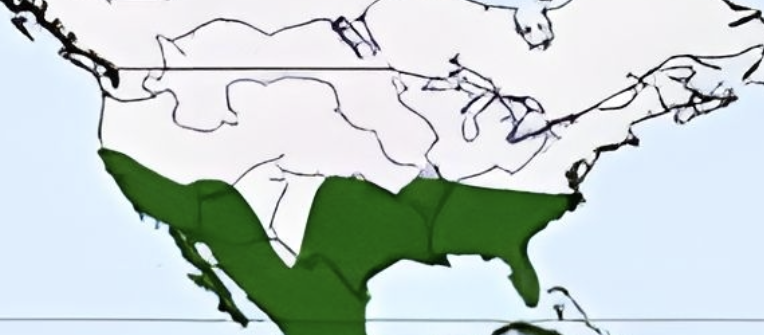
\includegraphics[width=\linewidth,height=3cm]{true_bat.png}
    \caption{True range of \textit{Tadarida Brasiliensis} (where green indicates presence) \cite{tbrasili_groms}
 }
    \label{fig:true-range}
\end{minipage}\hfill
\begin{minipage}[t]{0.48\linewidth}
    \centering
    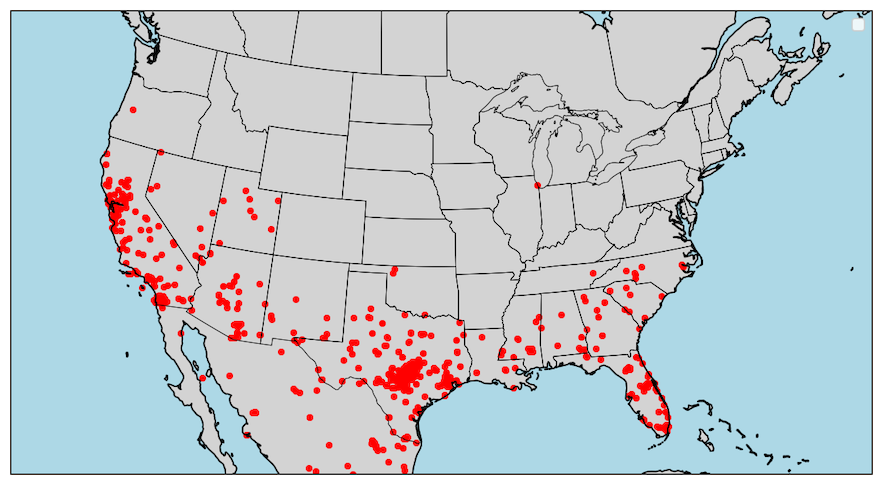
\includegraphics[width=\linewidth,height=3.1cm]{correct_bat.png}
    \caption{Observed range of \textit{Tadarida Brasiliensis}, where each point indicates an observation}
    \label{fig:correct_bat}
\end{minipage}
\end{figure}

The goal of this project is to predict the results of Figure \ref{fig:true-range} using SDMs and environmental data. Given the similarity between Figure \ref{fig:true-range} and Figure \ref{fig:correct_bat}, we have indication that our training data provides a relatively accurate representation of the true distribution of \textit{Tadarida Brasiliensis}, providing evidence of sufficient signal required to conduct our analysis. We note however that we are only investigating one species, and different species will have different distributions. \vspace{-0.4em}

\subsection{Feature Correlation}\vspace{-0.3em}

To investigate interdependence between climatic and geographic variables, a correlation heatmap was produced to assess pairwise correlations of our features (Figure \ref{fig:correlation matrix}). Note that the human population feature was not included in this visualisation, as it will be investigated in the subsequent section.

From Figure \ref{fig:correlation matrix}, we see that average soil moisture displayed  a strong correlation of 0.73, with mean precipitation. Due to the causal relationship between the variables, average soil moisture was excluded to reduce risk of multicollinearity.  Distance to coast and temperature variance also showed a high correlation of 0.73, which is logical since areas further inland tend to experience greater temperature variability. However, as these features capture distinct environmental mechanisms, we opted to keep both in our analysis. A similar rationale was applied for the strong correlations observed between the mean and variance of temperature and precipitation. \vspace{-0.2em}

\begin{figure}[H]
\begin{minipage}{0.48\linewidth}
    \centering
    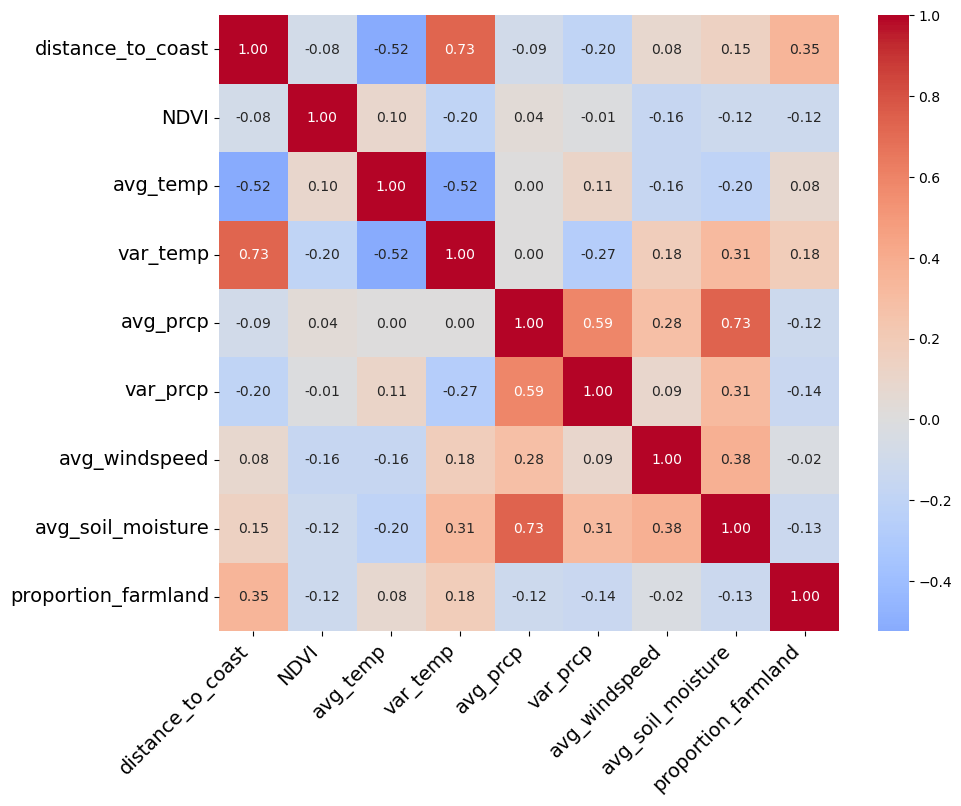
\includegraphics[width=0.95\linewidth]{plots/correlation matrix heatmap.png}
    \caption{Feature Correlation Matrix}
    \label{fig:correlation matrix}
\end{minipage}
\begin{minipage}{.48\linewidth}
    \centering
    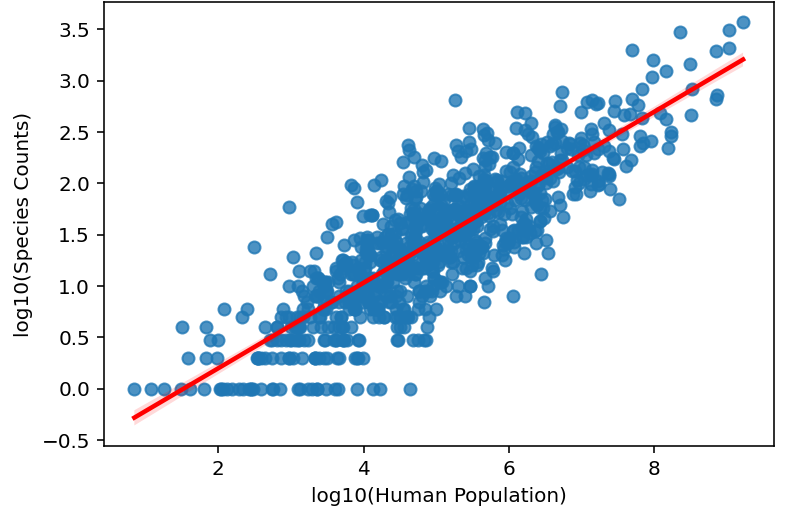
\includegraphics[width=0.9\linewidth]{lin_rel.png}
    \caption{Log-scaled human population and species counts per 1° × 1° Bin. Each blue point represents a 1° × 1° bin and the red line represents a fitted linear regression line}
    \label{lin_rel}
    \end{minipage}
\end{figure}\vspace{-0.6em}

\subsection{Human Population Analysis}\vspace{-0.3em}
\label{human pop anal}

According to a 2021 paper \cite{human_effect} regarding the trends and gaps in the use of citizen science for species distribution models, citizen science datasets are typically biased toward human population centers, areas that are easy to access, or regions frequented by active observers. This leads to over and under-sampled areas. Given that our data was collected via citizen science, we must account for potential sampling bias, and explore methods of mitigating this bias, before making conclusions from our results.

To investigate this potential bias, we first applied a logarithmic transformation to both human population and species observation counts per 1° × 1° bin of our data to reduce the influence of extreme values and stabilise the variance. To assess whether human population and species counts are related, we used this log-transformed data to fit a linear model.



After verifying the assumptions of linearity \cite{linear_assumptions} (see Appendix \ref{app:linearity}), we obtained Figure \ref{lin_rel}, which displays a clear linear relationship between our log-scaled population counts. We then obtained a Pearson correlation coefficient \cite{pearson_correlation} of 0.8387 and p-value<<0.05, which indicates that there is a statistically significant, positive log-linear relationship between human population and the number of species observations. 

Given these findings, we will not include human population as a model feature, as it would further amplify this sampling bias. The most common approach to generating absence data is to randomly generate absences uniformly across a geographic range. However, our findings demonstrate that species observations are influenced by human population, violating the assumption of uniformity. This finding prompts us to evaluate alternative methods for generating absence data.\vspace{-0.4em}

\section{Methods}\vspace{-0.4em}
\subsection{Modelling with Presence-Only Data}\vspace{-0.5em}


Our presence-only data lacks the negative targets required to carry out standard classification algorithms. The standard solution in academic papers on SDMs is to generate a set of species absence observations, known as pseudo-absences. A classification algorithm can then be trained as it would be for presence-absence data. Methods exist that do not require the fabrication of absence data, but have been shown to generally produce significantly poorer classifiers than methods using pseudo-absences \cite{Elith_2006} and thus will not be implemented in this study.

As mentioned in Section \ref{human pop anal}, the commonly-used method of generating absence data uniformly is not likely to capture the geographic bias in our citizen science data. Since more presence observations are observed in regions of high population density, it is likely there is a bias in the locations of those making observations rather than in the actual species distributions. We propose an alternative method for generating absence samples that takes into account this geographical bias: one-vs-rest pseudo-absence sampler. As absences, the sampler uniformly draws a set of specified size from all species presence observations corresponding to all other species. This is inspired by community models, which use information about all species to inform the classifier. In this report we will fit a range of classification models, using both methods of pseudo-absence generation. \vspace{-0.4em}


\subsection{Learning Models}\vspace{-0.4em}

Three classification models were implemented and analysed in this project; Logistic Regression (GLM), Random Forest (RF) and Gradient Boosted Decision Trees (GBDT). 

% we need to try to cut this down
\textbf{Logistic Regression} is a generalised linear model that uses a logit link function to transform a linear combination of the features (fitted by maximum likelihood estimation) to a probability of a positive result (classified as present if the probability is greater than a specified threshold). Only linear decision boundaries can be modelled, which may not be sufficiently expressive for our purposes. 
\textbf{Random Forest} (RF) is an ensemble method based on decision trees. Decision trees partition the feature space into regions using simple decision rules (selected using a greedy algorithm to maximise a set objective function); RFs build many trees on bootstrap samples and aggregate the trees' predictions (by averaging probabilities) to reduce overfitting. RFs typically display strong performance in species distribution modelling \cite{Elith_2022}, and can capture nonlinear relationships between the features and species presence. 
\textbf{Gradient Boosted Decision Trees} (GBDT) fit shallow decision trees successively, with each tree trained on the residual errors of the current model, and their contributions aggregated to form a final prediction. Boosting allows the model to retain a nonlinear decision boundary structure, and with sufficient regularisation can maintain good generalisation performance. GBDTs have been shown to perform well in species distribution modelling \cite{Elith_2006} and offer an alternative nonlinear method to RF. \vspace{-0.4em}

\subsection{Model Fitting}\vspace{-0.4em}
\label{hyperparams}
For each species with more than 1,000 presence observations (to ensure adequate data for model fitting), presence data was combined with generated pseudo-absence data (either through spatially uniform sampling or our one-vs-rest method), and were generated to be approximately equal to the number of presences. Logistic Regression, Random forest, and Gradient Boosting classifiers were trained on both one-vs-rest and uniformly generated pseudo-absence data. Hyperparameters were tuned through the use of 5-fold grid search cross validation \cite{GridSearch_CV} for each classification model, species and absence data type, where the metric to be maximised was the Area Under the Receiver Operating Characteristic Curve (AUC-ROC) on the validation set.

Justifying any given strategy for hyperparameter tuning on the validation set, including the method outlined above, is difficult due to the vastly different natures of the testing set and the validation set; it is not clear why evaluating any of the usual classification metrics on the validation set is a good measure of the generalisation error to the test set. We have therefore chosen to analyse both the tuned models and the default scikit-learn models in order to determine whether the hyperparameter tuning described above actually does captures any of the true generalisation error to the test set. \vspace{-0.4em}

\subsection{Evaluation Metrics}\vspace{-0.4em}
\label{AUCROC}
There is active discussion among ecologists about the most appropriate classification metric to use for SDMs. For example, while \cite{AUC_bad} raises some important issues with using AUC-ROC (such as a strong dependence on the area of study in relation to the true species range), \cite{Carpathians} argues for evaluating models based on AUC-ROC when paired with another metric such as cross-entropy. As AUC-ROC is  straightforward to calculate and remains the standard metric in practice, we follow the recommendation of \cite{Carpathians} by reporting both the AUC-ROC and cross entropy for each species and model. \vspace{-0.4em}

\section{Results}\vspace{-0.4em}

\begin{figure}[H] % this needs to be reformatted to be more readable
    \centering
    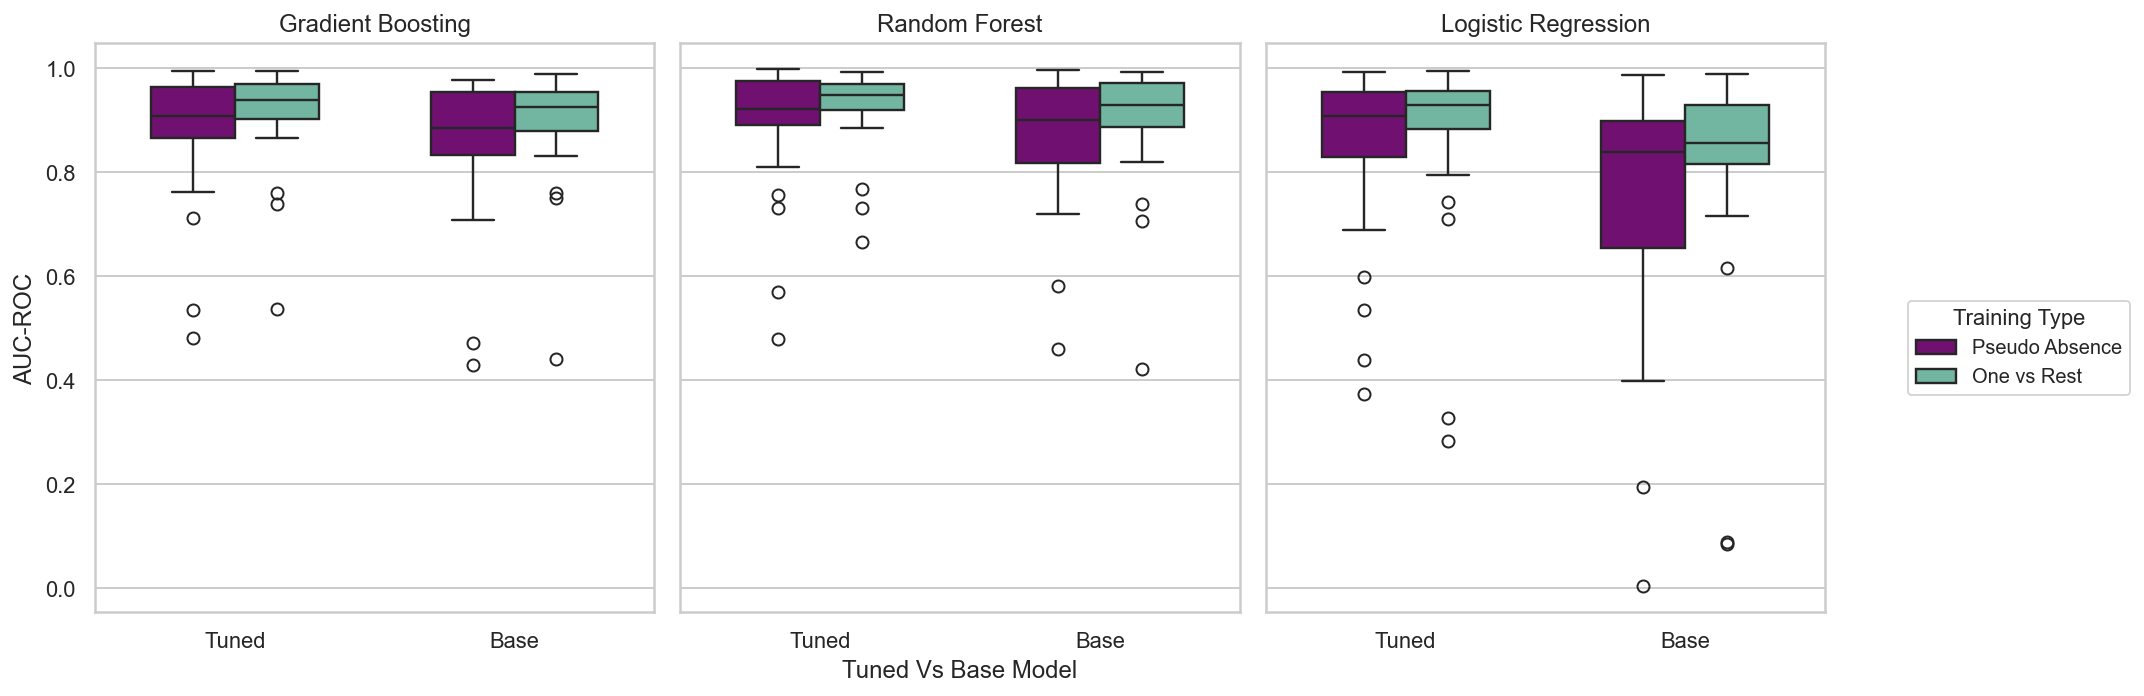
\includegraphics[width=1\linewidth]{resultsfig.png}
    \caption{Boxplots of AUC-ROC scores across different trained models}
    \label{fig:Results Fig}
\end{figure}
\subsection{Model results}\vspace{-0.4em}
For most species, the AUC-ROC scores of our models were generally high, and boxplots for the AUC-ROC scores across the 41 species for each pseudo-absence/model/hyperparameter tuning combination are displayed in Figure \ref{fig:Results Fig}. The best-performing model combination is tuned RF with one-vs-rest absence generation, achieving a mean AUC-ROC score of 0.932, closely followed by tuned GBDT with one-vs-rest absence generation with a mean AUC-ROC of 0.919. The logistic regression models performed significantly worse than the two tree ensembles, with the best of the four GLM models (tuned with one-vs-rest) achieving a mean AUC-ROC of 0.888. 


%The models perform very poorly on the same few species, notably the Northern Rough-winged Swallow, the House Wren and the Vesper Sparrow. 

The mean AUC-ROC of the models fitted on one-vs-rest pseudo-absence data consistently outperform models fitted on uniform pseudo-absences. This is true for all three classification models, both with base parameters and after tuning. A one-sided paired Wilcoxon signed-rank test \cite{Wilcoxon} was run for each model to determine if the difference in the location of the distributions of AUC-ROC scores for the different pseudo-absence generation methods was statistically significant. The results showed that this difference was significant at the 5\% significance level for all classification methods in both tuned and untuned forms. Table \ref{table:results} displays the results of these tests. This is further supported by the use of cross-entropy, in which the use of one-vs-rest resulted in a reduction of 0.34 for Gradient Boosting, 0.14 for Random Forest, and 0.14 for Logistic Regression in the average cross-entropy. 

Hyperparameter tuning resulted in only a moderate improvement in the mean performance of the models, with an average improvement of 0.031 in the mean AUC-ROC. We note that hyperparameter tuning also appears to mitigate the performance of the worst-performing models on the most difficult species to map. Hypothesis testing for pseudo-absence generation was conducted to assess whether tuned models performed significantly better than untuned models. At the 5\% significance level, all models were improved by hyperparameter tuning.

The use of random forests allow for the ability to quantify the importance of the features through the use of the Normalised Total Reduction of Entropy. It is important to note the significant variation in feature importance, demonstrating the importance of retraining our model for each species (as visualised in Appendix \ref{app:featureimportance}).


\begin{table}[h!]
\centering
\begin{tabular}{|l|l|l|l|}
\hline
Model & Type & \# species where 1vR beats uniform / 41 & p-value \\ \hline
GBDT & Tuned & 33 & $6.8 \times 10^{-6}$ \\ \hline
     & Base  & 31 & 0.00018 \\ \hline
RF   & Tuned & 26 & 0.0009 \\ \hline
     & Base  & 29 & 0.0003 \\ \hline
GLM  & Tuned & 23 & 0.0298 \\ \hline
     & Base  & 28 & 0.00035 \\ \hline
\end{tabular}
\vspace{6pt}  
\caption{Performance comparison of models using 1vR against uniform pseudo-absences}
\label{table:results}
\end{table}

\begin{figure}[t] 
\begin{minipage}{.48\linewidth}
\centering
    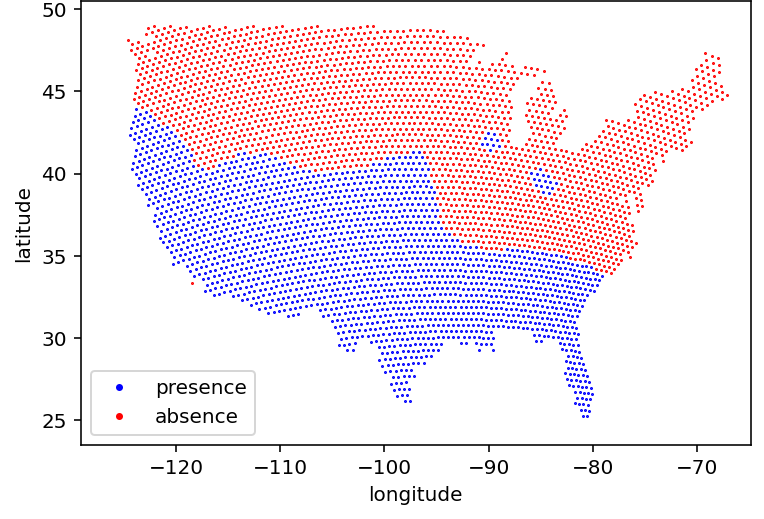
\includegraphics[width=\linewidth,height=3cm]{range_bat.png}
    \caption{Test set range of \textit{Tadarida Brasiliensis} \\ \\}
    \label{fig:Results Fig 3 }
    \end{minipage}
    \hfill
\begin{minipage}{.48\linewidth}
    \centering
    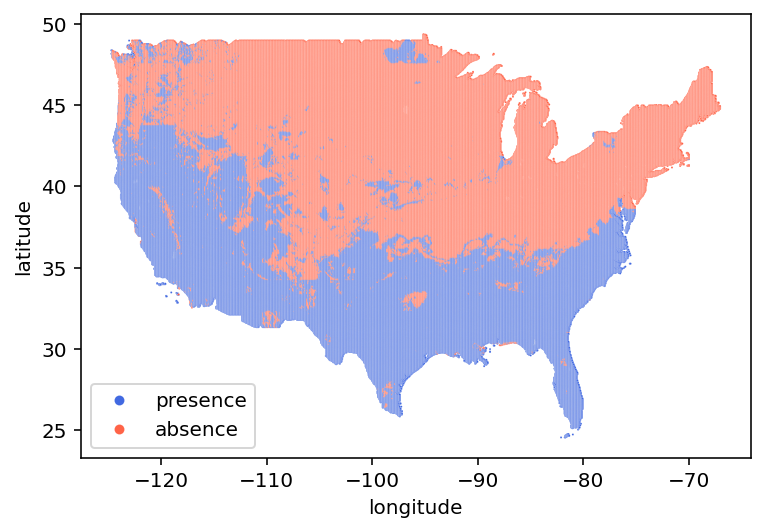
\includegraphics[width=\linewidth,height=3cm]{thresh2_bat.png}
    \caption{Predicted range of occurrence (using threshold 0.2) for \textit{Tadarida} \textit{Brasiliensis} (tuned one-vs-rest RF)}
    \label{fig:Results Fig 2 }
\end{minipage}    
\end{figure}\vspace{-1em}

\section{Discussion} \vspace{-0.4em}
The stronger performance of models trained on one-vs-rest pseudo-absences against those trained on uniform pseudo-absences is an important finding of this report, as it provides a simple method for counteracting bias in presence-only data. Our evidence for this positive effect is strong, with all six of the trained models showing evidence for this at the 5\% significance level. 

Our results give clear indication that tree-based ensemble methods give higher AUC-ROC results than Logistic Regression. This is in line with previous research \cite{Elith_2006}, and could result from the ensemble methods' ability to capture nonlinear decision boundaries. Our classification problem is unlikely to be solved well using linear decision boundaries, given that the habitable feature space for a given species will be some closed region, rather than some half-space. Linear classifiers such as Support Vector Machines (SVMs) are therefore unlikely to be effective in species distribution modelling. However, future investigation into non-linear methods such as Neural Networks may prove valuable.

While hypothesis testing confirms that hyperparameter tuning, as stated in Section \ref{hyperparams}, had a statistically significant effect on the test AUC-ROC of the resulting models, the effect is relatively modest for most of the models. As discussed in Section \ref{AUCROC}, this could be due to a limited ability of validation on the presence/generated absence data to estimate the error on the test set. Other methods designed for presence-only SDM evaluation, such as the spatial Boyce's Index \cite{Boyce}, could instead be used for validation, and may provide larger performance improvements. 

As seen in Figure \ref{fig:Results Fig}, there are significant outliers with regards to the AUC-ROC score. After investigating these outliers, we found that each involved a severe class imbalance in the test set, with far more presences than absences. 
When a species is present across the region, both the presence and absence data occupy the same environmental space. Therefore, the model gets very little signal about what separates areas where the species is present from areas where it is absent, and may predict an approximately constant presence probability. This suggests that our approach may not be suitable for species that occur across most of the training region. Despite the poor AUC-ROC score, these outlier species report a cross-entropy score of approximately 0.6, as would occur with an approximately constant 0.5 prediction probability.
\vspace{-0.4em}

\section{Conclusion}\vspace{-0.4em}
Fitting SDMs based on citizen science data required dealing with biased, presence-only data. We have generated pseudo-absence data using a one-vs-rest method to address geographical sampling bias, which was successful at improving the resulting distribution models over the standard, spatially uniform pseudo-absence generation. The best results were obtained using tuned decision tree ensembles, which were flexible enough to capture much of the complexity of the relationship between species presence and the environmental features. The tuned Random Forest and Gradient Boosting models trained on one-vs-rest pseudo-absences improved upon Logistic Regression trained on uniformly generated absences (our baseline model). These models achieved mean AUC-ROC scores on the test set of true species distributions of 0.932 and 0.919 respectively, a notable improvement over the baseline model's score of 0.854.
\newpage
\section*{Declaration of Generative AI Use}
In constructing our report, generative AI was used to aid us in loading and formatting external data, listed in Appendix \ref{app:environmental features}, into our code space. However, it was not used for any code generation or report-writing. 

\section*{Individual Member Contributions}
Each group member contributed a roughly equal amount across the entirety of the project. Group meetings were held for key idea generation, problem-solving discussions and final report editing.
Specifically, \textbf{s2274544} was involved in the collection of environmental feature data, writing of the introduction (Section 1), species data (Section 2.1) and external data (Section 2.2) analyses, SDM plausibility analysis (Section 3.1), and the human population analysis (Section 3.3).
\textbf{s2222962} was involved in the initial SDM research, implementing the models and absence generation methods, and write-ups in Section 4, 5, and 6.
\textbf{s2145762} wrote-up and implemented data collection methods specified in Section 2.2, as well as the write-up of Section 3.2, the nearest-neighbour matching analysis in Appendix A.2, and co-writing Section 4.2.
\textbf{s2859612} aided in the collection of the environmental feature data, wrote the code for implementing the training and testing of each model, result visualisations, feature importance and co-wrote Section 6. 

\newpage



\bibliography{refs.bib}
\bibliographystyle{plain}


\newpage
\appendix
%\section*{Appendix}

\section{External Data}
\subsection{Environmental Features}
\label{app:environmental features}

\begin{table}[H]
\centering
\begin{tabular}{|p{4cm}|p{6cm}|p{5cm}|}
\hline
\textbf{Feature Name} & \textbf{Info} & \textbf{Source} \\ \hline
Mean and Variance Temperature & 2020 Monthly Averages (°C) & National Centers for Environmental Information (NCEI) \\ \hline
Mean and Variance Surface Precipitation & 2020 Monthly Averages (mm) & National Centers for Environmental Information (NCEI)  \\ \hline
Mean Wind Speed & 2020 10m Above Ground (m/s) & National Centers for Environmental Information (NCEI) \\ \hline
Human Population & 2020 US City Populations & Simple Maps \\ \hline
Mean Soil Moisture & 2020 4xDaily Volumetric Soil Moisture 10cm Below Ground & National Centers for Environmental Information (NCEI) \\ \hline
Distance to Nearest Coastline & Minimum Distance from Observation to Coastline (in metres) & North American Cartographic Information Society (NACIS) \\ \hline
Normalised Difference Vegetation Index (NDVI) & 2020 Daily Averages, derived from the NOAA Climate Data Record (CDR) & National Centers for Environmental Information (NCEI) \\ \hline
Proportion of Surrounding Farmland Area & 2022 Proportion of Farmland by County & United States Department of Agriculture (USDA) \\ \hline
\end{tabular}
\caption{Environmental Features}
\end{table}


\subsection{Nearest-Neighbour Data Matching}
\label{app:nearest neighbours}
We now investigate the nearest-neighbour data matching process we perform to collect this external environmental data. The distances from each observation and its closest available data record are measured for each feature, and their cumulative distribution functions are plotted below. 

\begin{figure}[H]
    \centering
     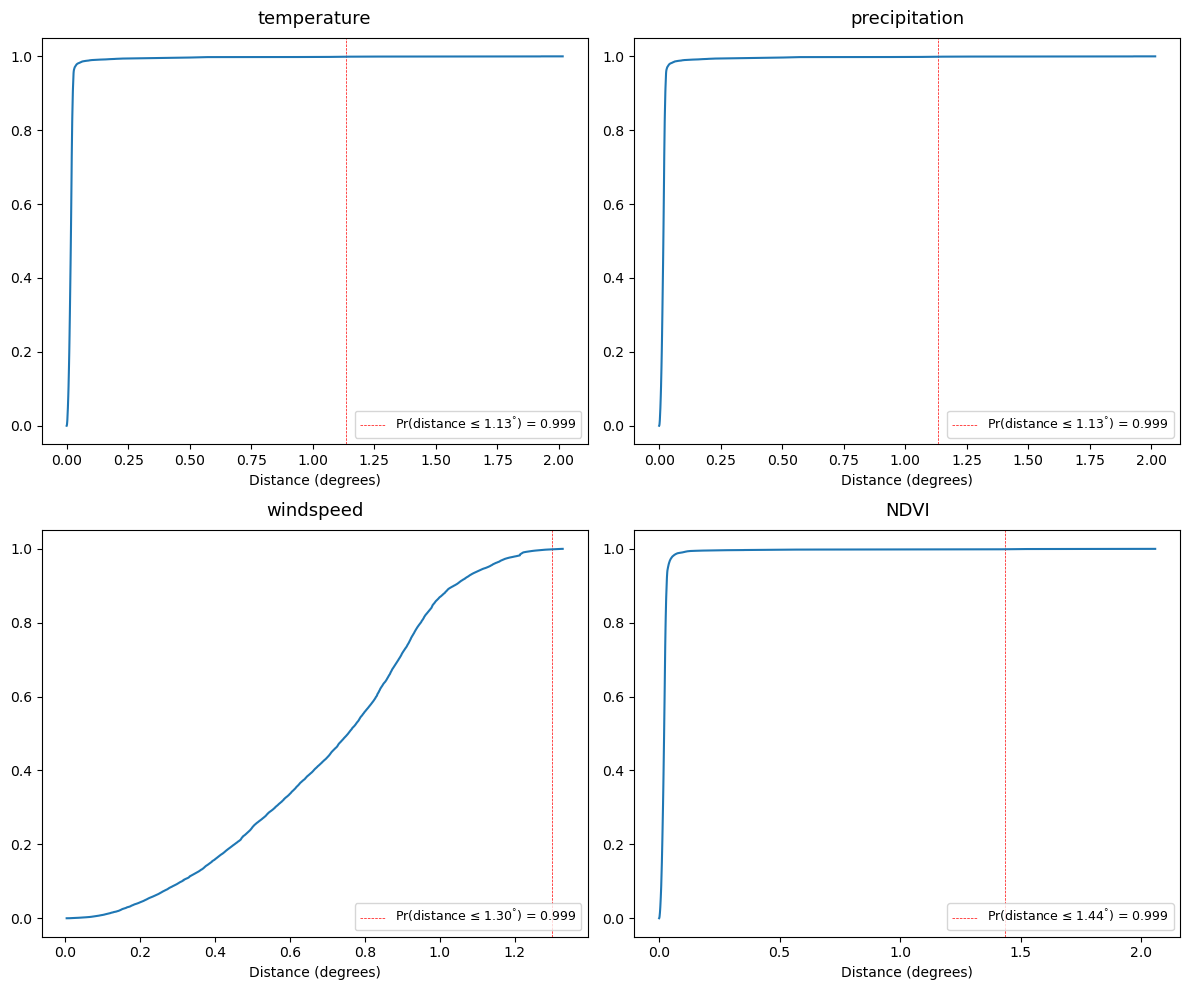
\includegraphics[width=0.7\linewidth]{plots/CDFs of distances.png}
    \caption{Cumulative Distribution Functions (CDFs) of Distances from observation to closest data record, for each respective feature}
    \label{fig:Distance CDFs}
\end{figure}

We find the mean distances from observation to data record for temperature, precipitation and NDVI data to be 0.0216$^\circ$, 0.0216$^\circ$ and 0.0249$^\circ$, respectively, while mean windspeed distance data is 0.7112$^\circ$ (to 4 decimal places), a significant difference. This is due to these data being collected from sources that use different grid-resolutions for extracting data. While temperature, precipitation and NDVI recordings are measured using sensor data projected on a 0.05$^\circ$ by 0.05$^\circ$ grid, windspeed is measured using reanalysed grid data, at a greater resolution of 1.9$^\circ$ by 1.9$^\circ$. Furthermore, while the windspeed distances seem to be more evenly distributed, the majority of temperature, precipitation and NDVI recordings are less than $1^\circ$, with only a small number of observations being a greater distance from the nearest climatic data. To further investigate this, we plot the observations where the distance of the data collection is greater than the 99.9th percentile of distances for each feature (see Figure \ref{fig:large distances}).
\begin{figure}[H]
    \centering
    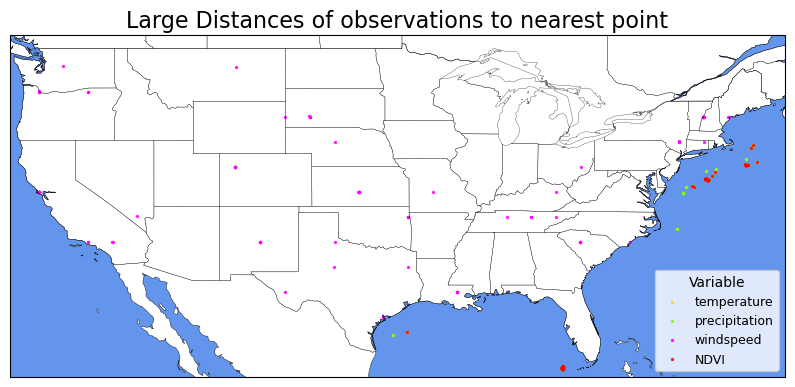
\includegraphics[width=0.7\linewidth]{plots/distances of species observations.png}
    \caption{Locations of observations where these large distances occur}
    \label{fig:large distances}
\end{figure}
We note from the plot that while our windspeed distances are fairly evenly spread across the US, our temperature, precipitation and NDVI large distances appear to almost entirely be observations recorded at sea.

To resolve this, we removed all observations that were recorded over one mile away from the United States mainland, reducing our observation count by 1060 to 84,358. 
In doing so, our mean distances from observation to data record for temperature, precipitation, NDVI and windspeed data are 0.0172$^\circ$, 0.0172$^\circ$, 0.0214$^\circ$, and 0.7109$^\circ$ (to 4 decimal places), respectively. We also note that the maximum distance from observation to record decreased by 44\% for temperature and precipitation data and decreased by 29\% for NDVI data.






\section{Exploratory Data Analysis}
\subsection{Human vs. Species Linearity Assumptions}
\label{app:linearity}


\begin{figure}[H]
\begin{minipage}[t]{0.48\linewidth}
    \centering
    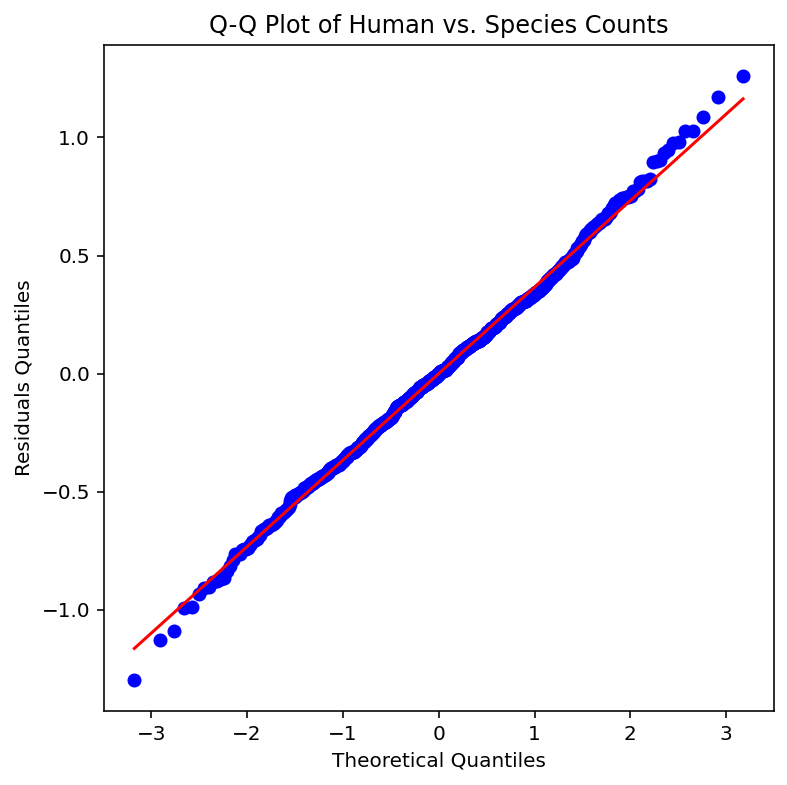
\includegraphics[width=\linewidth, height=5cm]{qq.png}
    \caption{Q-Q plot of residuals from the linear regression of log10(Species Counts) on log10(Human Population).}
    \label{fig:qq}
\end{minipage}\hfill
\begin{minipage}[t]{0.48\linewidth}
    \centering
    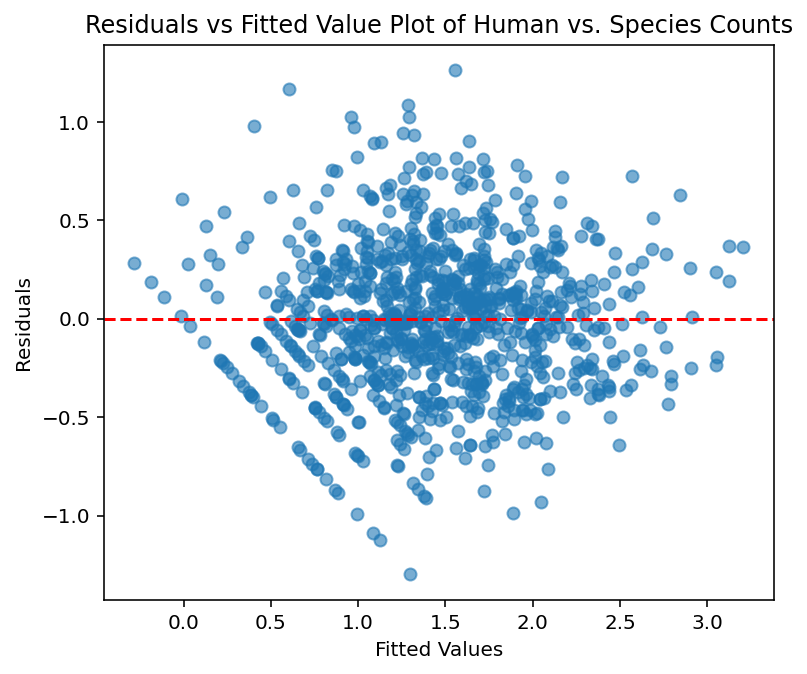
\includegraphics[width=\linewidth, height=5cm]{res_vs_fitted.png}
    \caption{Residuals vs Fitted Values for Linear Regression of log10(Species Counts) on log10(Human Population)}
    \label{fig:res_vs_fitted}
\end{minipage}
\end{figure}

Given that the residual points are located closely around the red reference line in Figure \ref{fig:qq}, we have indication that our residuals follow the normality assumption. Additionally, given how the blue points in Figure \ref{fig:res_vs_fitted} are scattered relatively randomly around 0, we have indication that the residuals have constant mean and variance.

\section{Results}
\subsection{Feature Importance}
\label{app:featureimportance}

\begin{figure}[H]
    \centering
    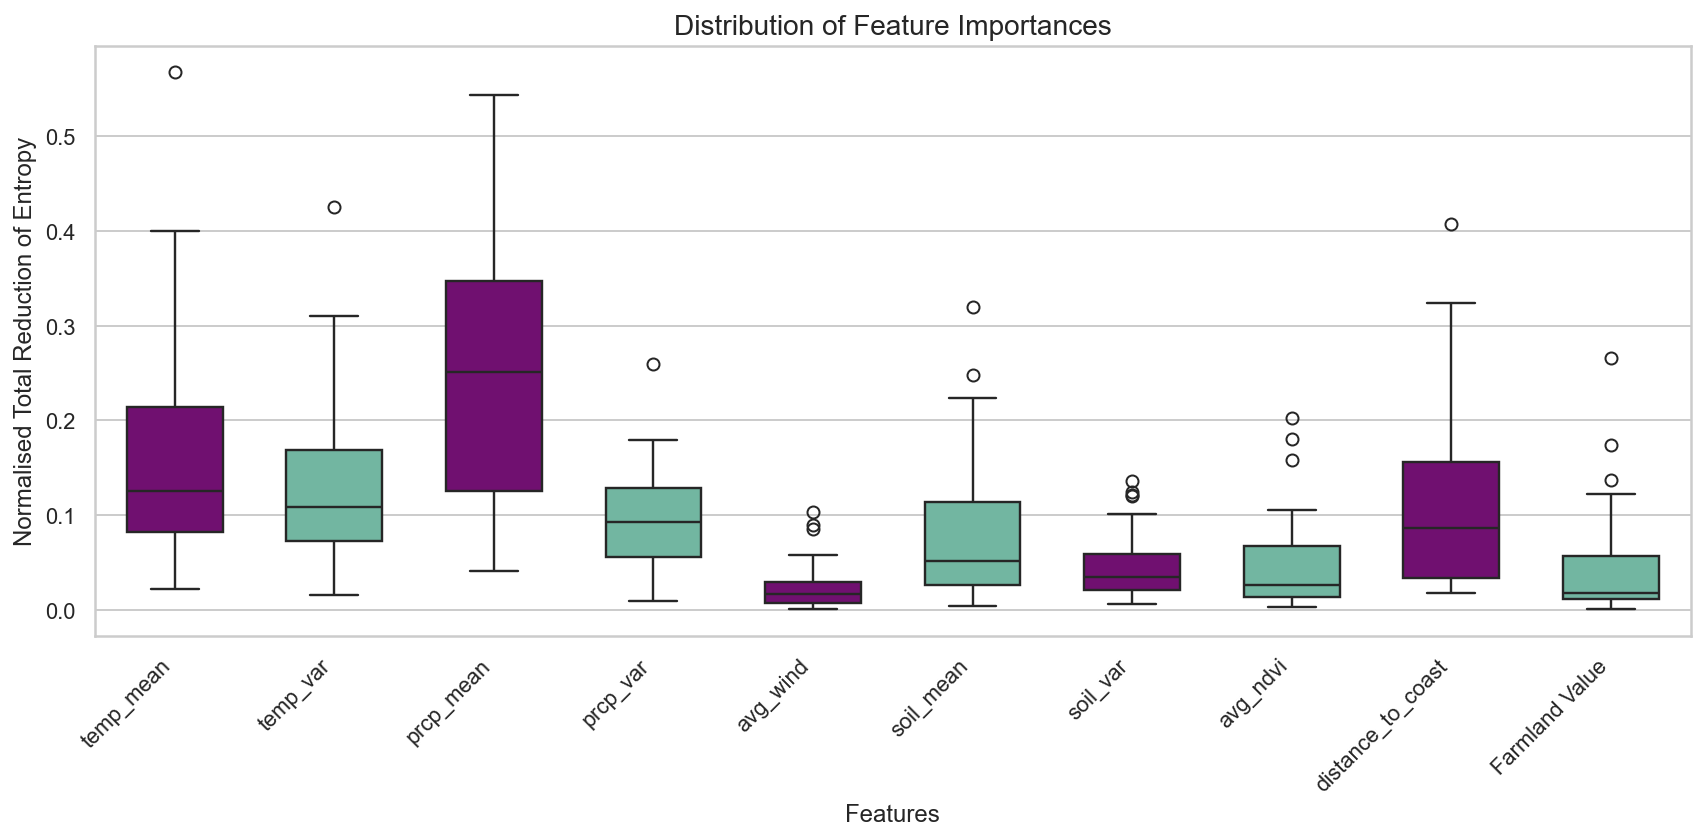
\includegraphics[width=1\linewidth]{feature importance 2 .png}
    \caption{Feature Importance}
    \label{fig: feature importance}
\end{figure}

% Evaluation:
% E1: https://www.nature.com/articles/s41598-020-80062-1
% E2: https://www.sciencedirect.com/science/article/pii/S1574954124004588


\end{document}

%%% Local Variables:
%%% mode: latex
%%% TeX-master: t
%%% End: